\documentclass{standalone}
\usepackage{tikz}
\usetikzlibrary{patterns, positioning}


\begin{document}
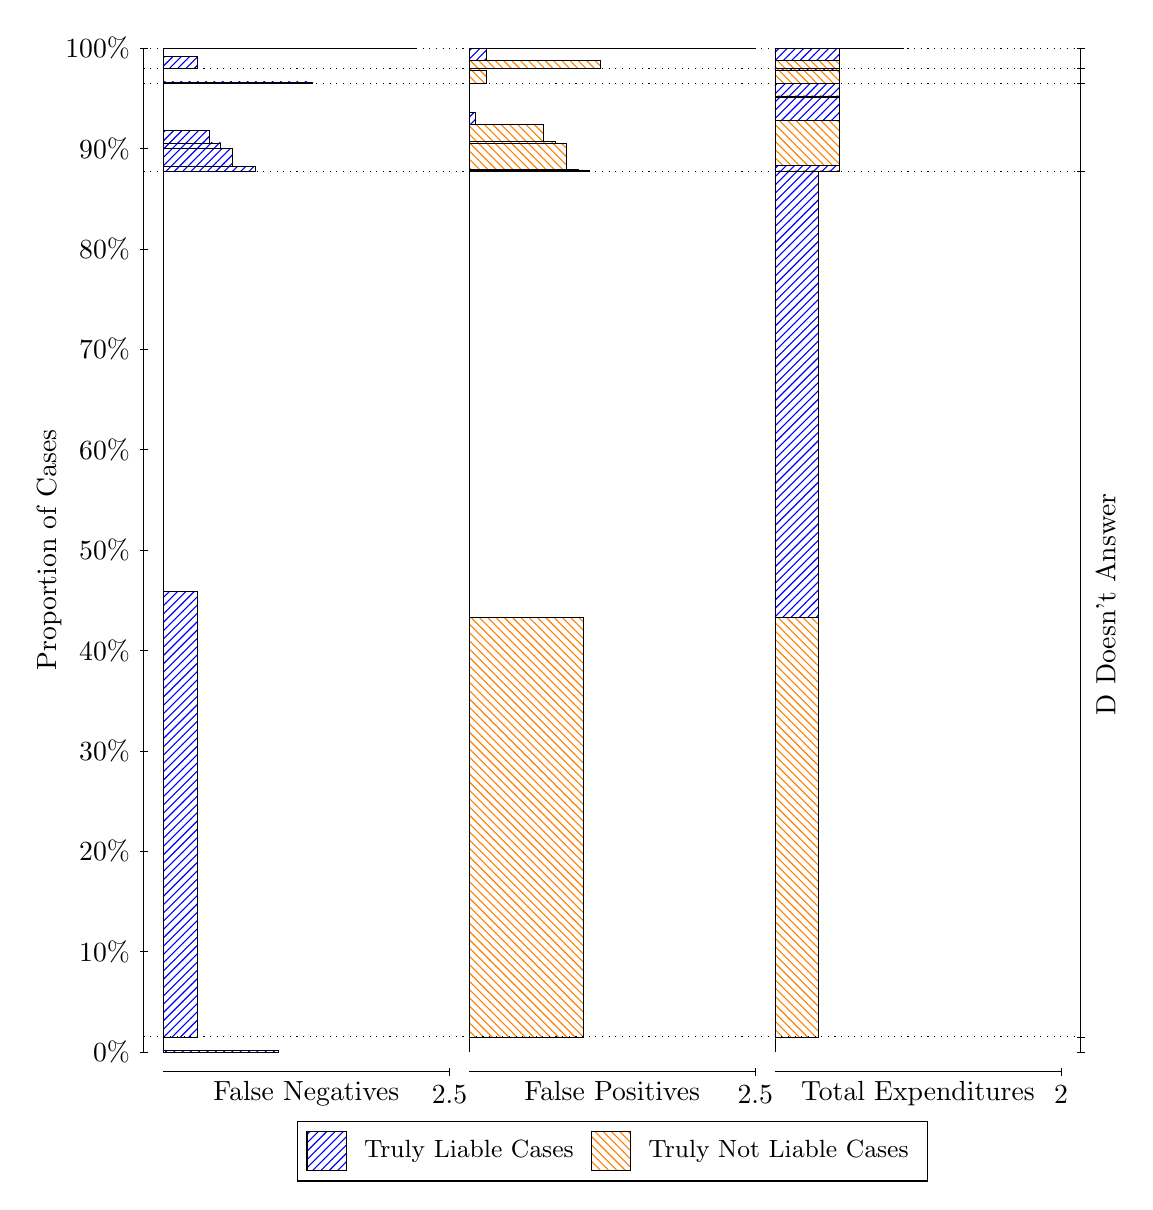
\begin{tikzpicture}
\draw[black, very thin] (1.5,1.75) -- (1.5,14.5);
\node[rotate=90, text=black, anchor=center] at (0.3, 8.125) {Proportion of Cases};
\draw[black, very thin] (1.45,1.75) -- (1.55,1.75);
\node[text=black, anchor=east] at (1.45, 1.75) {0\%};
\draw[black, very thin] (1.45,3.025) -- (1.55,3.025);
\node[text=black, anchor=east] at (1.45, 3.025) {10\%};
\draw[black, very thin] (1.45,4.3) -- (1.55,4.3);
\node[text=black, anchor=east] at (1.45, 4.3) {20\%};
\draw[black, very thin] (1.45,5.575) -- (1.55,5.575);
\node[text=black, anchor=east] at (1.45, 5.575) {30\%};
\draw[black, very thin] (1.45,6.85) -- (1.55,6.85);
\node[text=black, anchor=east] at (1.45, 6.85) {40\%};
\draw[black, very thin] (1.45,8.125) -- (1.55,8.125);
\node[text=black, anchor=east] at (1.45, 8.125) {50\%};
\draw[black, very thin] (1.45,9.4) -- (1.55,9.4);
\node[text=black, anchor=east] at (1.45, 9.4) {60\%};
\draw[black, very thin] (1.45,10.675) -- (1.55,10.675);
\node[text=black, anchor=east] at (1.45, 10.675) {70\%};
\draw[black, very thin] (1.45,11.95) -- (1.55,11.95);
\node[text=black, anchor=east] at (1.45, 11.95) {80\%};
\draw[black, very thin] (1.45,13.225) -- (1.55,13.225);
\node[text=black, anchor=east] at (1.45, 13.225) {90\%};
\draw[black, very thin] (1.45,14.5) -- (1.55,14.5);
\node[text=black, anchor=east] at (1.45, 14.5) {100\%};

\draw[black, very thin] (13.4,1.75) -- (13.4,14.5);
\draw[black, very thin] (13.35,1.75) -- (13.45,1.75);
\node[anchor=west] at (13.35, 1.75) {};
\draw[black, very thin] (13.35,1.9424) -- (13.45,1.9424);
\node[anchor=west] at (13.35, 1.9424) {};
\draw[black, very thin] (13.35,12.929) -- (13.45,12.929);
\node[anchor=west] at (13.35, 12.929) {};
\draw[black, very thin] (13.35,14.049) -- (13.45,14.049);
\node[anchor=west] at (13.35, 14.049) {};
\draw[black, very thin] (13.35,14.243) -- (13.45,14.243);
\node[anchor=west] at (13.35, 14.243) {};
\draw[black, very thin] (13.35,14.492) -- (13.45,14.492);
\node[anchor=west] at (13.35, 14.492) {};
\draw[black, very thin] (13.35,14.497) -- (13.45,14.497);
\node[anchor=west] at (13.35, 14.497) {};
\draw[black, very thin] (13.35,14.5) -- (13.45,14.5);
\node[anchor=west] at (13.35, 14.5) {};

\draw[black, very thin, pattern color=blue, pattern=north east lines] (1.75,1.75) rectangle (3.2033,1.7702);
\draw[black, very thin, pattern color=orange, pattern=north west lines] (1.75,1.7702) rectangle (1.75,1.9424);
\draw[black, very thin, pattern color=blue, pattern=north east lines] (1.75,1.9424) rectangle (2.186,7.5983);
\draw[black, very thin, pattern color=orange, pattern=north west lines] (1.75,7.5983) rectangle (1.75,12.929);
\draw[black, very thin, pattern color=blue, pattern=north east lines] (1.75,12.929) rectangle (2.9127,12.994);
\draw[black, very thin, pattern color=blue, pattern=north east lines] (1.75,12.994) rectangle (2.7673,12.997);
\draw[black, very thin, pattern color=blue, pattern=north east lines] (1.75,12.997) rectangle (2.622,13.224);
\draw[black, very thin, pattern color=blue, pattern=north east lines] (1.75,13.224) rectangle (2.4767,13.294);
\draw[black, very thin, pattern color=blue, pattern=north east lines] (1.75,13.294) rectangle (2.3313,13.45);
\draw[black, very thin, pattern color=orange, pattern=north west lines] (1.75,13.45) rectangle (1.75,14.049);
\draw[black, very thin, pattern color=blue, pattern=north east lines] (1.75,14.049) rectangle (3.6393,14.07);
\draw[black, very thin, pattern color=orange, pattern=north west lines] (1.75,14.07) rectangle (1.75,14.243);
\draw[black, very thin, pattern color=blue, pattern=north east lines] (1.75,14.243) rectangle (2.186,14.396);
\draw[black, very thin, pattern color=orange, pattern=north west lines] (1.75,14.396) rectangle (1.75,14.492);
\draw[black, very thin, pattern color=blue, pattern=north east lines] (1.75,14.492) rectangle (4.9473,14.493);
\draw[black, very thin, pattern color=orange, pattern=north west lines] (1.75,14.493) rectangle (1.75,14.497);
\draw[black, very thin, pattern color=orange, pattern=north west lines] (1.75,14.497) rectangle (1.75,14.499);
\draw[black, very thin, pattern color=blue, pattern=north east lines] (1.75,14.499) rectangle (1.75,14.5);
\draw[black, very thin, pattern color=orange, pattern=north west lines] (5.6333,1.75) rectangle (5.6333,1.9222);
\draw[black, very thin, pattern color=blue, pattern=north east lines] (5.6333,1.9222) rectangle (5.6333,1.9424);
\draw[black, very thin, pattern color=orange, pattern=north west lines] (5.6333,1.9424) rectangle (7.0867,7.2732);
\draw[black, very thin, pattern color=blue, pattern=north east lines] (5.6333,7.2732) rectangle (5.6333,12.929);
\draw[black, very thin, pattern color=orange, pattern=north west lines] (5.6333,12.929) rectangle (7.1593,12.948);
\draw[black, very thin, pattern color=orange, pattern=north west lines] (5.6333,12.948) rectangle (7.014,12.959);
\draw[black, very thin, pattern color=orange, pattern=north west lines] (5.6333,12.959) rectangle (6.8687,13.288);
\draw[black, very thin, pattern color=orange, pattern=north west lines] (5.6333,13.288) rectangle (6.7233,13.317);
\draw[black, very thin, pattern color=orange, pattern=north west lines] (5.6333,13.317) rectangle (6.578,13.528);
\draw[black, very thin, pattern color=blue, pattern=north east lines] (5.6333,13.528) rectangle (5.706,13.684);
\draw[black, very thin, pattern color=blue, pattern=north east lines] (5.6333,13.684) rectangle (5.6333,14.049);
\draw[black, very thin, pattern color=orange, pattern=north west lines] (5.6333,14.049) rectangle (5.8513,14.221);
\draw[black, very thin, pattern color=blue, pattern=north east lines] (5.6333,14.221) rectangle (5.6333,14.243);
\draw[black, very thin, pattern color=orange, pattern=north west lines] (5.6333,14.243) rectangle (7.3047,14.339);
\draw[black, very thin, pattern color=blue, pattern=north east lines] (5.6333,14.339) rectangle (5.8513,14.492);
\draw[black, very thin, pattern color=orange, pattern=north west lines] (5.6333,14.492) rectangle (5.6333,14.496);
\draw[black, very thin, pattern color=blue, pattern=north east lines] (5.6333,14.496) rectangle (5.6333,14.497);
\draw[black, very thin, pattern color=orange, pattern=north west lines] (5.6333,14.497) rectangle (9.2667,14.499);
\draw[black, very thin, pattern color=blue, pattern=north east lines] (5.6333,14.499) rectangle (7.8133,14.5);
\draw[black, very thin, pattern color=orange, pattern=north west lines] (9.5167,1.75) rectangle (9.5167,1.9222);
\draw[black, very thin, pattern color=blue, pattern=north east lines] (9.5167,1.9222) rectangle (9.5167,1.9424);
\draw[black, very thin, pattern color=orange, pattern=north west lines] (9.5167,1.9424) rectangle (10.062,7.2732);
\draw[black, very thin, pattern color=blue, pattern=north east lines] (9.5167,7.2732) rectangle (10.062,12.929);
\draw[black, very thin, pattern color=orange, pattern=north west lines] (9.5167,12.929) rectangle (10.334,12.94);
\draw[black, very thin, pattern color=blue, pattern=north east lines] (9.5167,12.94) rectangle (10.334,13.01);
\draw[black, very thin, pattern color=orange, pattern=north west lines] (9.5167,13.01) rectangle (10.334,13.579);
\draw[black, very thin, pattern color=blue, pattern=north east lines] (9.5167,13.579) rectangle (10.334,13.874);
\draw[black, very thin, pattern color=orange, pattern=north west lines] (9.5167,13.874) rectangle (10.334,13.893);
\draw[black, very thin, pattern color=blue, pattern=north east lines] (9.5167,13.893) rectangle (10.334,14.049);
\draw[black, very thin, pattern color=orange, pattern=north west lines] (9.5167,14.049) rectangle (10.334,14.221);
\draw[black, very thin, pattern color=blue, pattern=north east lines] (9.5167,14.221) rectangle (10.334,14.243);
\draw[black, very thin, pattern color=orange, pattern=north west lines] (9.5167,14.243) rectangle (10.334,14.339);
\draw[black, very thin, pattern color=blue, pattern=north east lines] (9.5167,14.339) rectangle (10.334,14.492);
\draw[black, very thin, pattern color=orange, pattern=north west lines] (9.5167,14.492) rectangle (11.152,14.496);
\draw[black, very thin, pattern color=blue, pattern=north east lines] (9.5167,14.496) rectangle (11.152,14.497);
\draw[black, very thin, pattern color=orange, pattern=north west lines] (9.5167,14.497) rectangle (11.152,14.499);
\draw[black, very thin, pattern color=blue, pattern=north east lines] (9.5167,14.499) rectangle (11.152,14.5);
\draw[black, dotted] (1.5,1.9424) -- (13.4,1.9424);
\draw[black, dotted] (1.5,12.929) -- (13.4,12.929);
\draw[black, dotted] (1.5,14.049) -- (13.4,14.049);
\draw[black, dotted] (1.5,14.243) -- (13.4,14.243);
\draw[black, dotted] (1.5,14.492) -- (13.4,14.492);
\draw[black, dotted] (1.5,14.497) -- (13.4,14.497);
\draw[black, very thin] (1.75,1.5) -- (5.3833,1.5);
\node[text=black, anchor=north] at (3.5667, 1.5) {False Negatives};
\draw[black, very thin] (5.3833,1.45) -- (5.3833,1.55);
\node[text=black, anchor=north] at (5.3833, 1.45) {2.5};

\draw[black, very thin] (5.6333,1.5) -- (9.2667,1.5);
\node[text=black, anchor=north] at (7.45, 1.5) {False Positives};
\draw[black, very thin] (9.2667,1.45) -- (9.2667,1.55);
\node[text=black, anchor=north] at (9.2667, 1.45) {2.5};

\draw[black, very thin] (9.5167,1.5) -- (13.15,1.5);
\node[text=black, anchor=north] at (11.333, 1.5) {Total Expenditures};
\draw[black, very thin] (13.15,1.45) -- (13.15,1.55);
\node[text=black, anchor=north] at (13.15, 1.45) {2};


\node[text=black, centered, rotate=90] at (13.72, 7.4357) {D Doesn't Answer};






\draw (7.449999999999999,1.5) node[draw=none] (baseCoordinate) {};
\begin{scope}[align=center]
        \matrix[scale=0.5, draw=black, below=0.5cm of baseCoordinate, nodes={draw}, column sep=0.1cm]{
            \node[rectangle, draw, minimum width=0.5cm, minimum height=0.5cm, pattern color=blue, pattern=north east lines] {}; &
            \node[draw=none, font=\small, text=black] (B) {Truly Liable Cases}; &
            \node[rectangle, draw, minimum width=0.5cm, minimum height=0.5cm, pattern color=orange, pattern=north west lines] {}; &
            \node[draw=none, font=\small, text=black] (B) {Truly Not Liable Cases}; \\
            };
\end{scope}

\end{tikzpicture}
\end{document}